Figure~\ref{fig:piep_architecture} presents an overview of the \sys{} architecture. \sys{}
first decomposes the LLM into individual constituent modules (\S\ref{ss:design-decomposition}), allowing \sys{} to directly model the energy consumption of compute and communication in parallel inference.
Since the number of GPUs involved in parallel inference influences the energy consumption and tensor shapes of individual modules, \sys{} makes use of resource- and architecture-aware features for each module based on the parallelization strategy (\S\ref{ss:design-features}).
\sys{} then explicitly predicts the energy used for GPU communication (\S\ref{ss:design-communication}) and carefully measures both computation and communication energy to collect ground truth (\S\ref{ss:design-measurement}).
Finally, \sys{} builds a multi-level regressor to combine these contributions to accurately learn end-to-end energy (\S\ref{ss:design-prediction}).

\begin{figure*}[t]
\centering
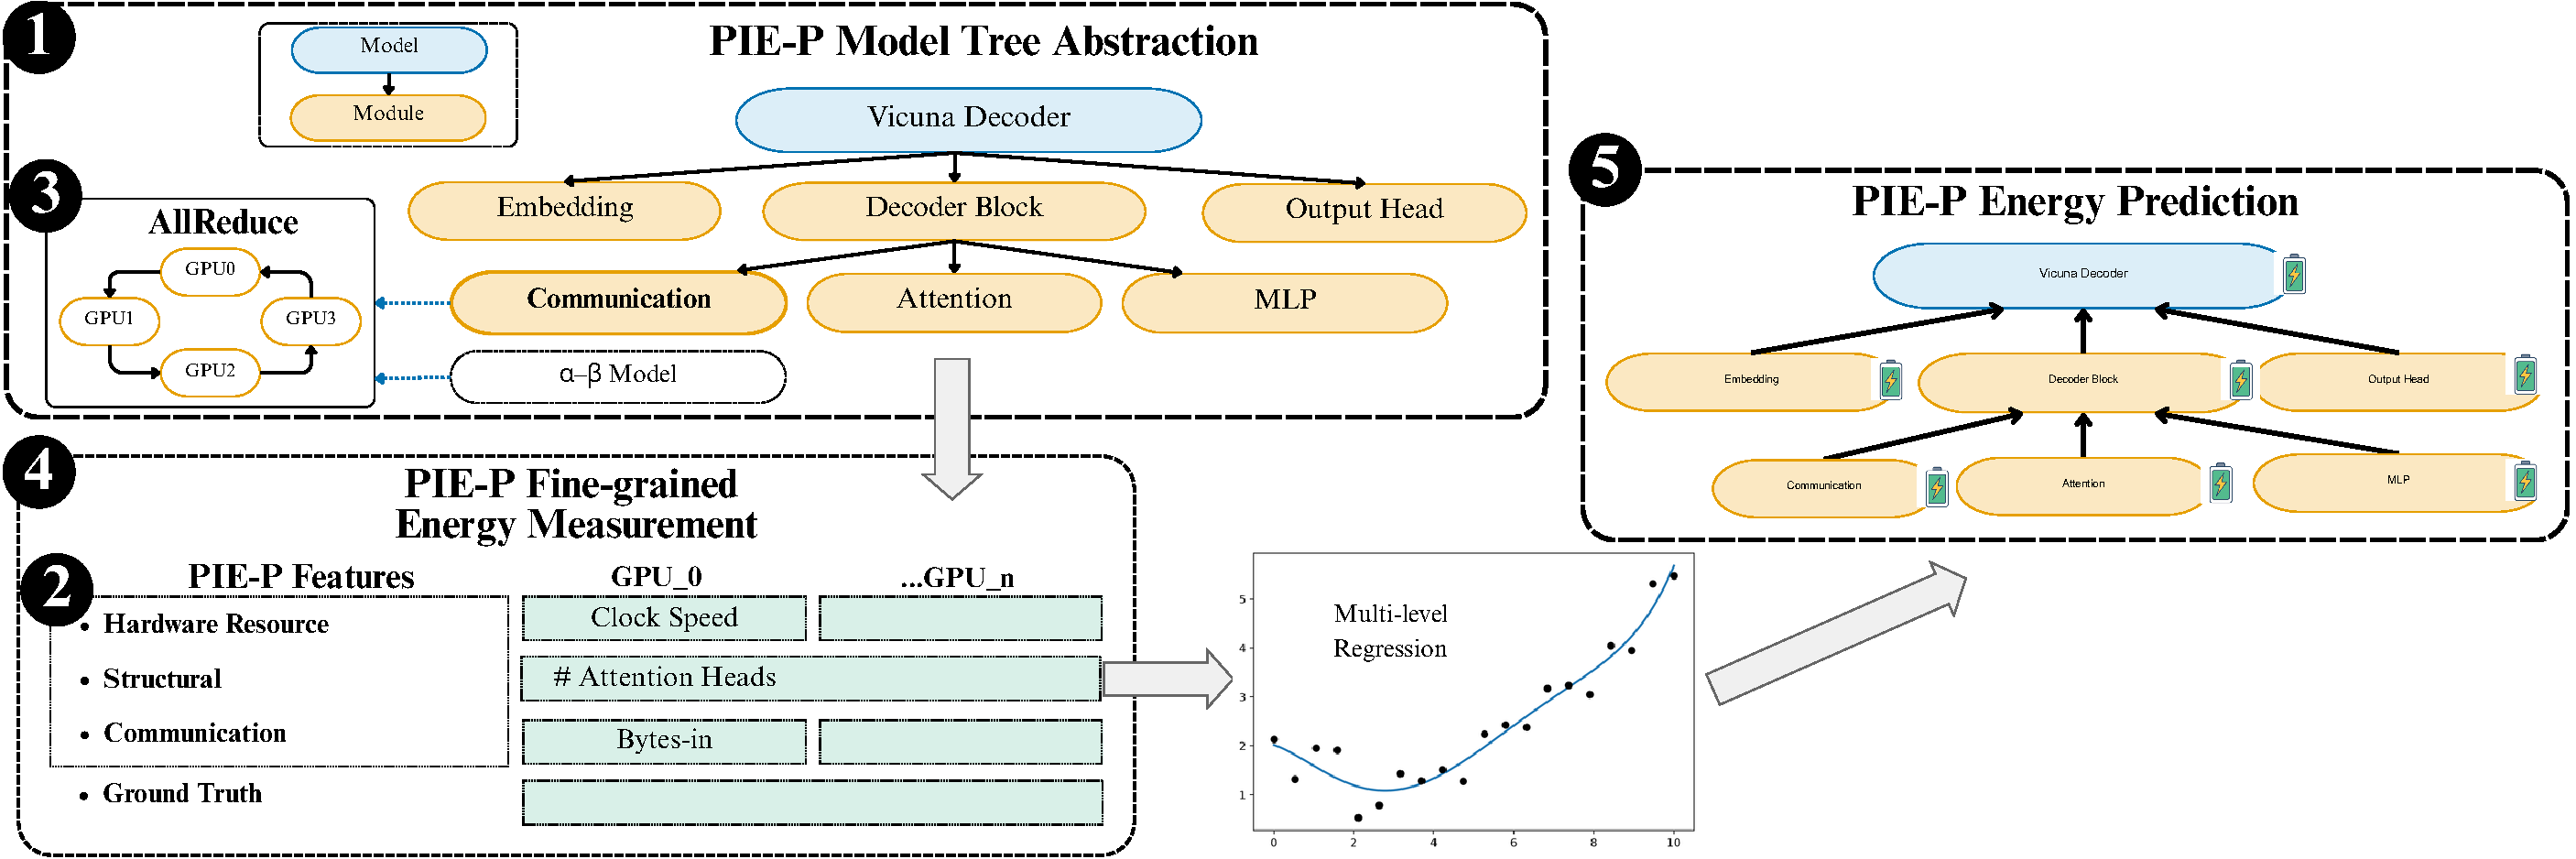
\includegraphics[
    width=\textwidth,
    height=0.20\textheight,
    keepaspectratio
]{figures/piepv6.pdf}
\vspace{-9pt}
\caption{\sys{} architecture showing: (1) parallelism-aware decomposition, (2) features for module-level prediction, (3) communication energy modeling, (4) measurement and data collection, and (5) multi-level regression.}
\label{fig:piep_architecture}
\vspace{-18pt}
\end{figure*}

\subsection{Parallelism-Aware Decomposition into Compute and Communication Modules}
\label{ss:design-decomposition}

\sys{} uses a \emph{model-tree abstraction}, a graph-structured representation to decompose the inference run into constituent units (i.e., modules). Unlike prior work (e.g., IrEne~\cite{irene}) that only focuses on compute modules, the \sys{} model tree decomposes a model using both compute \emph{and} communication modules.

Concretely, \sys{} represents an LLM inference run as a hierarchical composition of modules, where each Transformer block is decomposed into child modules (e.g., AllReduce, Attention, MLP, normalization, embedding, output).
For inter-GPU communication, such as AllReduce operations, \sys{} adds a separate communication module to the model tree and records the data transferred between GPUs (see Figure~\ref{fig:piep_architecture}); this is then used to predict communication energy as discussed in \S\ref{ss:design-communication}.
This decomposition into modules can be obtained from existing ML frameworks, including PyTorch (using \texttt{torch.fx} symbolic tracing) or TensorFlow (using graph tracing).

\subsection{Features for Module-Level Prediction}
\label{ss:design-features}

To capture the relationship between energy and the compute and communication modules, \sys{} leverages hardware resource, model execution, and model structural features.
For example, the \emph{number of attention heads} influences how work is divided across GPUs during tensor parallelization, affecting communication volume in AllReduce operations.
We thus extract such structural features from the model for parallelized energy prediction; existing utilization- or metrics-based heuristics~\cite{strubell19,Nguyen-hotcarbon,wilkins2024offlineenergyoptimalllmserving} miss out on this critical information.

\begin{table}[t]
\centering
\small
\setlength{\tabcolsep}{4pt}
\renewcommand{\arraystretch}{1.05}
\begin{tabular}{@{}
>{\raggedright\arraybackslash}p{0.48\linewidth}
>{\raggedright\arraybackslash}p{0.48\linewidth}
@{}}
\toprule
\rowcolor{rowblue}
\multicolumn{2}{@{}l@{}}{\textbf{Resource Utilization Features}}\\
\midrule
CPU utilization (\%) & CPU mem. utilization (\%)\\
\rowcolor{rowblue} GPU utilization (\%) & GPU mem. utilization (\%)\\
CPU clock (GHz) & CPU mem. clock (GHz)\\
\rowcolor{rowblue} Memory (bytes) & GPU clock (GHz)\\
GPU mem. clock (GHz) & \\
\midrule
\rowcolor{rowblue}
\multicolumn{2}{@{}l@{}}{\textbf{Execution Features}}\\
\midrule
Batch size & Sequence length\\
\rowcolor{rowblue} FLOPs per token (billions) & Execution time (s)\\
GPU energy NVML (Wh) & Number of GPUs\\
\midrule
\rowcolor{rowblue}
\multicolumn{2}{@{}l@{}}{\textbf{Model Structure Features}}\\
\midrule
Feed-forward dimension & Transformer blocks\\
\rowcolor{rowblue} Hidden embedding size & Attention heads\\
Key--value heads & \\
\midrule
\rowcolor{rowblue}
\multicolumn{2}{@{}l@{}}{\textbf{Communication Features}}\\
\midrule
Bytes transferred & Effective bandwidth\\
\bottomrule
\end{tabular}
\caption{Features used by \sys{} for prediction.}
\label{tab:features}
\end{table}

Table~\ref{tab:features} summarizes the complete feature set.
Resource utilization features capture system- and device-level activity during inference; execution features capture the workload configuration that drives runtime and energy; and model-structure features capture architectural properties that determine tensor sizes.
For communication modules, \sys{} additionally uses the amount of data transferred and the effective bandwidth of each inter-GPU communication event.
A Spearman analysis across Vicuna configurations further shows that total energy correlates not only with NVML GPU energy ($\rho=0.633$--$0.762$), but also with batch size ($\rho=0.735$--$0.737$), execution time ($\rho=0.658$--$0.664$), and memory usage ($\rho=0.656$--$0.663$), motivating the use of multiple runtime and structural features rather than a single utilization signal.

\subsection{Communication Energy Modeling}
\label{ss:design-communication}

To model the communication energy introduced by parallel inference, \sys{} first treats inter-GPU communication events as explicit modules in the model tree.
For each communication event $e$, we trace the communication tensor sizes and calculate network transfer bytes sent ($B_{e}^{\mathrm{out}}$) and received ($B_{e}^{\mathrm{in}}$) by each GPU and use an offline-calibrated $\alpha$--$\beta$ model~\cite{hockney1988parallel2} to estimate the communication latency as:

\vspace{-12pt}
\begin{equation}
\label{eq:comm-latency-main}
T_{e}^{\mathrm{comm}} =
\alpha_{o,p} +
\beta_{o,p}
\left(
B_{e}^{\mathrm{out}} + B_{e}^{\mathrm{in}}
\right),
\end{equation}
\vspace{-8pt}
where $o$ denotes the communication operation (e.g., AllReduce or point-to-point transfer), $p$ is the number of GPUs, $\alpha_{o,p}$ captures the fixed communication overhead, and $\beta_{o,p}$ captures the message-size-dependent transfer cost.
For each event, we define the per-GPU communication volume as $V_e=B_e^{\mathrm{out}}+B_e^{\mathrm{in}}$.

We calibrate $\alpha_{o,p}$ and $\beta_{o,p}$ offline for each communication operation and GPU count by recording the observed communication time and volume across calibration runs and fitting $T_e^{\mathrm{obs}}=\alpha_{o,p}+\beta_{o,p}V_e$.
The corresponding effective bandwidth is $B^{\mathrm{eff}}_{o,p}=1/\beta_{o,p}$.
For ring AllReduce, a tensor of size $S_e$ bytes results in a per-GPU communication volume of
\begin{equation}
V_e^{\mathrm{AR}} = \frac{2(p-1)}{p}S_e,
\label{eq:allreduce_volume}
\end{equation}
accounting for both the ReduceScatter and AllGather phases.
For pipeline-parallel point-to-point transfers and data-parallel AllGather operations, we compute the communication volume from the transferred tensor size using the corresponding communication pattern.

Finally, \sys{} converts the predicted communication latency to communication-module energy by multiplying it with the calibrated average communication power $\bar{P}^{\mathrm{comm}}_{o,p}$:
\begin{equation}
\widehat{E}^{\mathrm{comm}}_e =
\bar{P}^{\mathrm{comm}}_{o,p} T_e^{\mathrm{comm}}.
\label{eq:comm_energy}
\end{equation}
The resulting communication-module estimate is then composed with the compute-module estimates by the multi-level regressor described in \S\ref{ss:design-prediction}.

\subsection{Measurement and Data Collection}
\label{ss:design-measurement}

\sys{} measures communication energy by first identifying the communication events introduced by each parallelism strategy and then isolating the corresponding windows in the execution trace. We align these communication windows with the system power trace and integrate power over the corresponding intervals to obtain communication-energy measurements for training the communication-module predictor. Effective bandwidth is computed from the observed communication volume and transfer time, while bytes sent and received are derived from the tensor size being communicated.

The communication window is identified differently for each parallelism strategy. \textbf{Tensor parallelism:} we profile ring AllReduce repeatedly to capture the distribution of synchronization and communication energy caused by non-deterministic leading and lagging GPU behavior. The profiled window includes both hop transfers and synchronization stalls across the ReduceScatter and AllGather phases. \textbf{Pipeline parallelism:} for each stage boundary, we use \texttt{nsys} to timestamp the end of stage $i$'s last forward kernel and the start of stage $i{+}1$'s first forward kernel; the intervening interval is attributed to the point-to-point activation transfer, and power is integrated over this window. \textbf{Data parallelism:} replicas execute their local forward passes independently and perform a tail-end AllGather to collate final outputs; we profile this final output stage to measure the corresponding communication energy.

For compute modules, \sys{} records (i) resource-specific signals that summarize system/GPU activity and (ii) model-specific descriptors extracted from the LLM configuration.
\sys{} collects repeated offline measurements for each module across controlled execution runs to build a stable training dataset for the module-level regressors (\S\ref{ss:design-prediction}). This captures non-deterministic straggler effects in observed communication behavior and improves the stability of the learned regressors. Because all profiling and calibration are performed offline, \sys{} incurs no additional measurement overhead during inference.

\subsection{Multi-Level Regression}
\label{ss:design-prediction}

Our methodology for training regressors follows a hierarchical approach, training module-level predictors and then combining them for model-level prediction.
As \sys{} obtains features from multiple GPUs, naively learning separate coefficients per GPU does not scale as the number of parameters grows with GPU count.
Instead, \sys{} computes statistical aggregates of runtime features using the mean, standard deviation, minimum, and maximum across all GPUs. These are combined with the static structural features to form the complete feature vector for each sample.

\sys{} uses the following multi-level regression formulation:
\vspace{-6pt}
\begin{equation}
\small
\begin{aligned}
P_e(m) &=
\sum_{c \in \mathcal{C}(m)} \alpha(c)\,P_e(c),\\[2pt]
P_e(c) &=
f_{\mathrm{Module}(c)}\!\left(\mathrm{feat}(c)\right)
\quad \text{if } c \text{ is a compute module},\\[2pt]
P_e(c) &=
\bar{P}^{\mathrm{comm}}_{o(c),p}\,
T_{c}^{\mathrm{comm}}
\quad \text{if } c \text{ is a communication module},\\[3pt]
\alpha(c) &=
1 + \frac{\tanh(\mathbf{W}\,\mathrm{feat}(c)+b)}{\tau}.
\end{aligned}
\label{eqn:end2end-predicted-sum}
\vspace{-7pt}
\end{equation}

Eq.~(\ref{eqn:end2end-predicted-sum}) defines the final model-level prediction. Here, $P_e(m)$ denotes the predicted end-to-end energy of model $m$, and $\mathcal{C}(m)$ is the set of compute and communication modules.
For a compute module $c$, $P_e(c)$ is predicted using the module-specific regression function $f_{\mathrm{Module}(c)}$; in our implementation, this is a decision-tree regressor trained separately for each module type.
For a communication module $c$, $P_e(c)$ is computed as the average observed communication power $\bar{P}^{\mathrm{comm}}_{o(c),p}$ multiplied by the communication time $T_{c}^{\mathrm{comm}}$ obtained from Eq.~\eqref{eq:comm-latency-main}. The average communication power is calibrated for communication operation type $o(c)$ (e.g., AllReduce, AllGather) and GPU count $p$.
Finally, $\alpha(c)$ is the learned composition weight for module $c$.
This formulation makes the bottom-up prediction explicit: \sys{} first predicts the energy of compute and communication modules, then combines those module-level predictions to obtain the model-level energy $P_e(m)$.

This hierarchical composition enables \emph{cross-variant and cross-model reuse} since many modules (e.g., Attention and MLP blocks) are shared across different models. While we do not claim generalization to arbitrary architectures, our results in \S\ref{sec:model_prediction} demonstrate that \sys{} generalizes across multiple model families.
